% !TeX spellcheck = it_IT
\newpage
\section{Concorrenza}
Il sistema operativo deve gestire molte cose contemporaneamente (\textbf{MTAO} - Multiple Things at Once): processi, interrupts, manutenzione di background, etc...
Non è solo il SO che deve gestire tutti questi aspetti, ma anche \emph{server} (garantire più connessioni simultanee), \emph{programmi} (migliori performance), \emph{interfacce} (aumentare la responsiveness), \emph{network} e \emph{dischi} (ridurre la latenza).

\begin{note}
	Il parallelismo è quando del codice può essere eseguito effettivamente nello stesso momento mentre la concorrenza è più virtuale: è lo scheduler che alterna i processi.
\end{note}

\subsection{Inter-Process Communication}
La concorrenza porta i processi ad avere un loro spazio di memoria riservato e si rende quindi necessario un \textbf{Inter-Process Communication} (IPC) per scambiare le informazioni e sincronizzarsi. C'è quindi un maggiore \emph{overhead} di comunicazione.
\begin{center}
	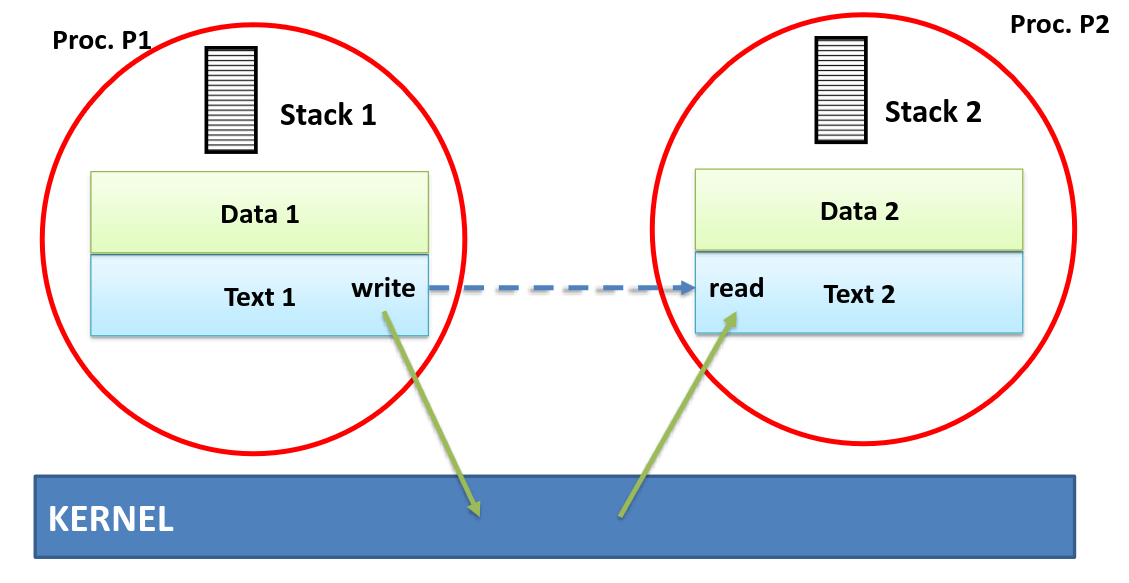
\includegraphics[scale=0.3]{ipc.png}
\end{center}


\subsection{Thread}
I thread sono singole entità che eseguono una \textbf{task indipendente} (può essere messa in pausa del SO). Condividono la memoria del processo che li crea, poiché fanno parte dello stesso spazio di memoria, ed eseguono un pezzo di codice. \\
Il vantaggio principale è il fatto che non si deve più passare dal SO per comunicare e c'è quindi un vantaggio \textbf{prestazionale}. Inoltre migliora l'\textbf{organizzazione} della struttura codice.

\subsubsection{Protezione}
Rimane che il thread può accedere solamente alla memoria del suo processo, garantendo così la protezione. C'è però da prestare attenzione ad evitare che un thread acceda ai dati di un altro thread nello stesso processo. In questo caso si SO non rileva errori. Eventuali tecniche di protezione sono implementate allo user-level dal RTS.
\begin{center}
	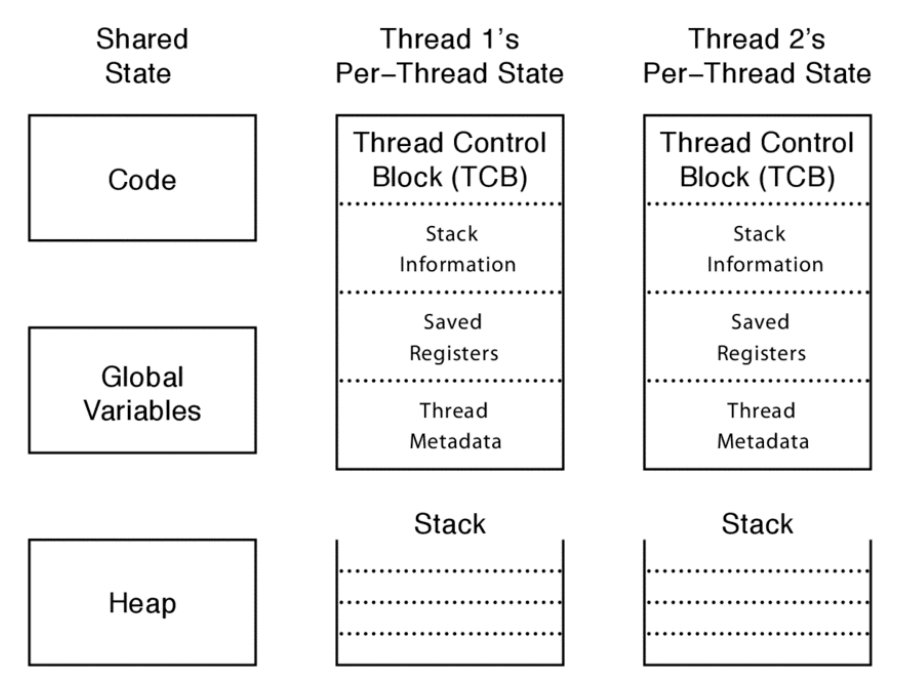
\includegraphics[scale=0.2]{thread_protection.png}
\end{center}

\subsubsection{Astrazione}
Ogni processo può creare virtualmente infiniti thread. Lo sviluppatore non sa in che ordine e con che velocità verrà poi eseguito ognuno di essi, dato che viene gestito dal kernel, e deve quindi progettare il software in modo che possa funzionare indipendentemente dalla schedule.
\begin{center}
	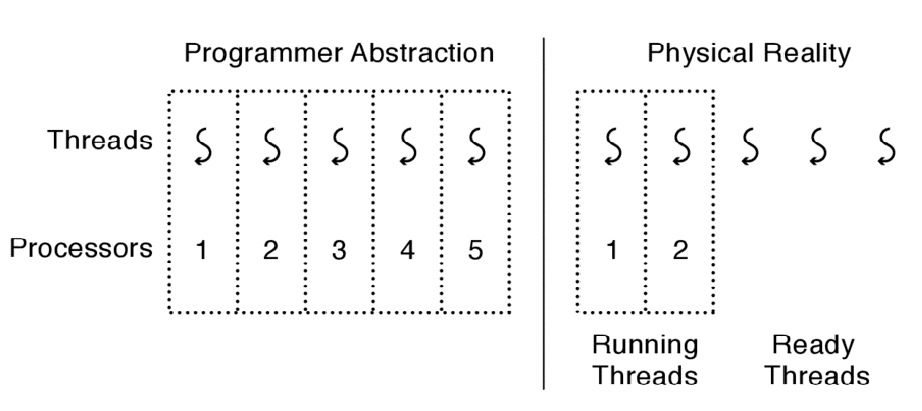
\includegraphics[scale=0.2]{thread_abstraction.png}
\end{center}

\subsubsection{Implementazione}
Alla base dei thread troviamo il \textbf{Thread Control Block} (TCB), ovvero una struttura dati che contiene le informazioni necessarie al thread., quali:
\begin{itemize}
	\item Thread ID
	\item Stato
	\item Contesto del thread
	\item Parametri di scheduling
	\item Riferimenti allo stack
\end{itemize}
È importante definire le \textbf{operazioni} sui thread e uno \textbf{scheduler}, ovvero una funzione del sistema operativo che si occupi di assegnargli dei processori.\\
Lo scheduler viene mandato in esecuzione periodicamente dal SO tramite degli interrupt attivati dal \textbf{timer}:
\begin{center}
	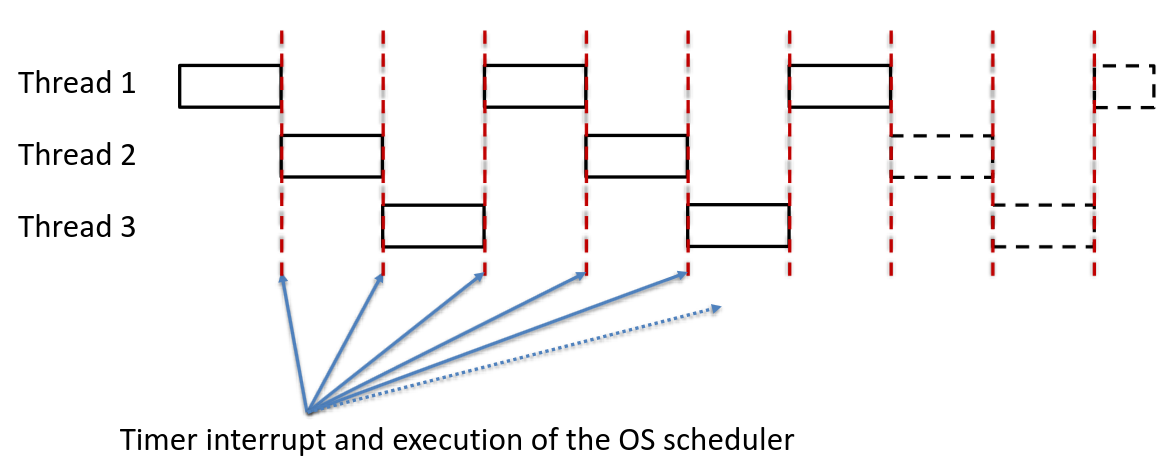
\includegraphics[scale=0.3]{thread_scheduler.png}
\end{center}
Distinguiamo due tipi di thread:
\begin{itemize}
	\item \textbf{Cooperative}: \label{thread_types}cooperano tra di loro in modo esplicito, ovvero con particolari istruzioni viene controllato lo scheduler. Finché non viene dato un comando o finché non scade il timer, rimane attivo quel thread
	\item \textbf{Preemptive}: partono e possono essere fermati dal SO in qualunque momento
\end{itemize}
che possono essere implementati in modi diversi:
\begin{itemize}
	\item Processi multipli \textbf{single-threaded}
	\item Processi multipli all'interno di un singolo processo, dove lo scheduler è gestito da una libreria (\textbf{user-level threads})
	\item \textbf{Misto} tra single e multi-threaded (\textbf{kernel-level threads})
	\item \textbf{Scheduler activation}
\end{itemize}

\subsubsection{API}
\begin{itemize}
	\item \textbf{create(thread, func, args)}: crea un thread e lo salva in \emph{thread}, poi esegue \emph{func} con gli argomenti in \emph{args}
	\item \textbf{yield()}: il thread smette volontariamente di usare il processore per dare spazio ad altri
	\item \textbf{join(thread)}: attende che il \emph{thread} finisca e a quel punto restituisce lo stato di uscita
	\item \textbf{exit(status)}: termina il thread corrente con un determinato \emph{status} 
\end{itemize}

\subsubsection{Ciclo di vita}
\begin{center}
	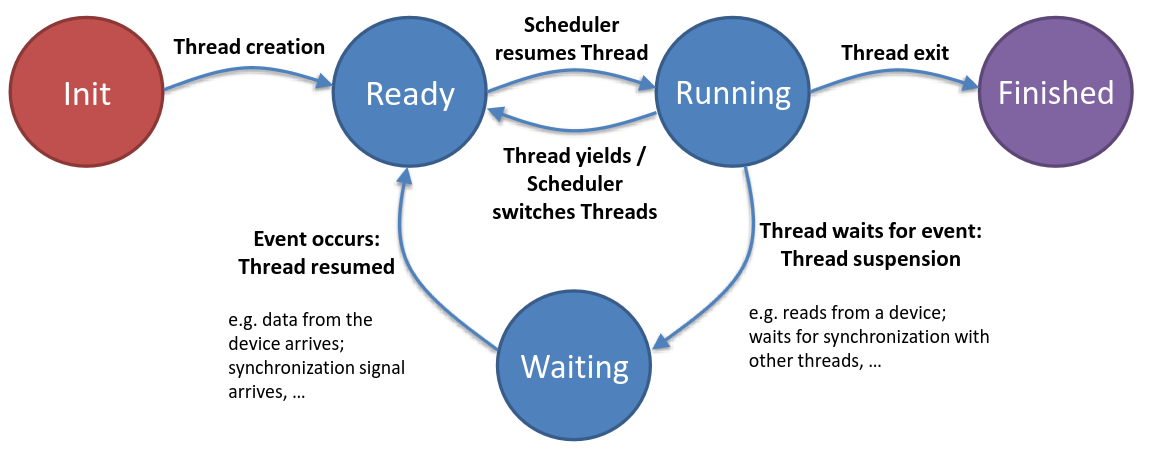
\includegraphics[scale=0.3]{thread_lifecycle.png}
\end{center}
Tutti questi stati sono implementati tramite \textbf{code} (liste). Ogni stato ha diverse code.
\begin{note}
	Un altro possibile caso in cui il thread passa dallo stato \emph{running} a quello \textit{ready} è quando abbiamo uno scheduler con una politica di tipo \textit{preemptive} e il SO crea un nuovo processo con priorità maggiore.
\end{note}

Nella seguente tabella è indicato dove si trovano i registri in ogni stato del ciclo di vita. 
\begin{center}
	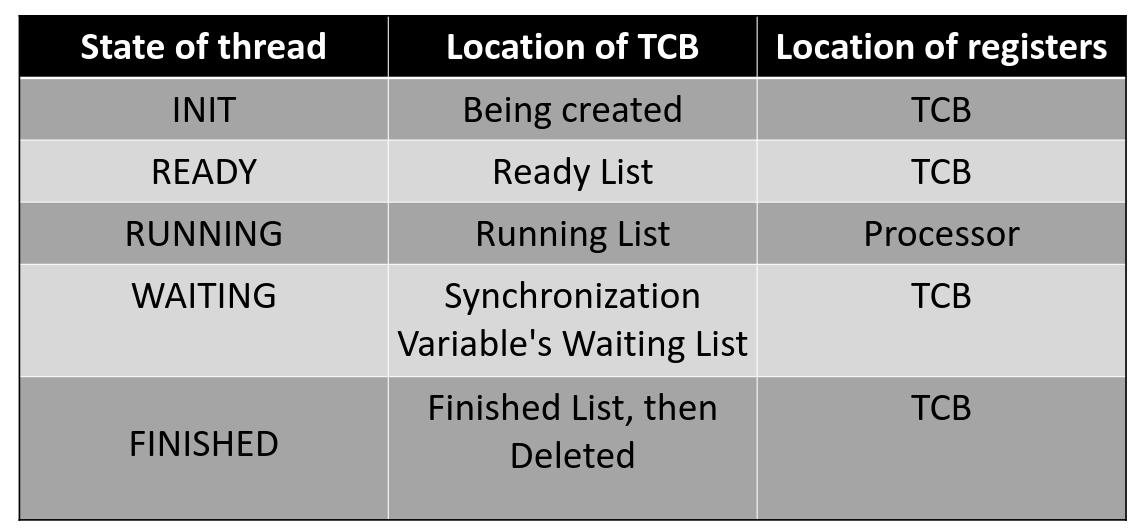
\includegraphics[scale=0.2]{tcb_register.png}
\end{center}
Riassumendo, l'unico caso in cui i registri non sono quelli del TCB, è quando il thread è in esecuzione, poiché in quel momento i registri validi sono nel processore.
\subsubsection{User-level thread}
Sono implementati a livello utente, ovvero il SO non è a conoscenza del fatto che un determinato processo sia al suo interno formato da più thread logici. Lo scheduling è quindi fatto da una libreria a livello utente: il \textbf{Run Time Support} (RTS).\\
Il modello utilizzato in questo schema è quello \textbf{cooperativo} (vedi \ref{thread_types}). Potrebbe essere implementato anche con il modello \textbf{preemptive} utilizzando le \emph{Scheduler Activation} di Windows o le \emph{UpCall}.\\
Le problematiche principali sono:
\begin{itemize}
	\item La mancanza di conoscenza da parte del SO mi impedisce di sfruttare a pieno le risorse del sistema
	\item Quando invoco una \textbf{system-call bloccante}, viene bloccato l'intero processo, dato che il SO non sa cosa c'è dentro al processo
\end{itemize}
\begin{center}
	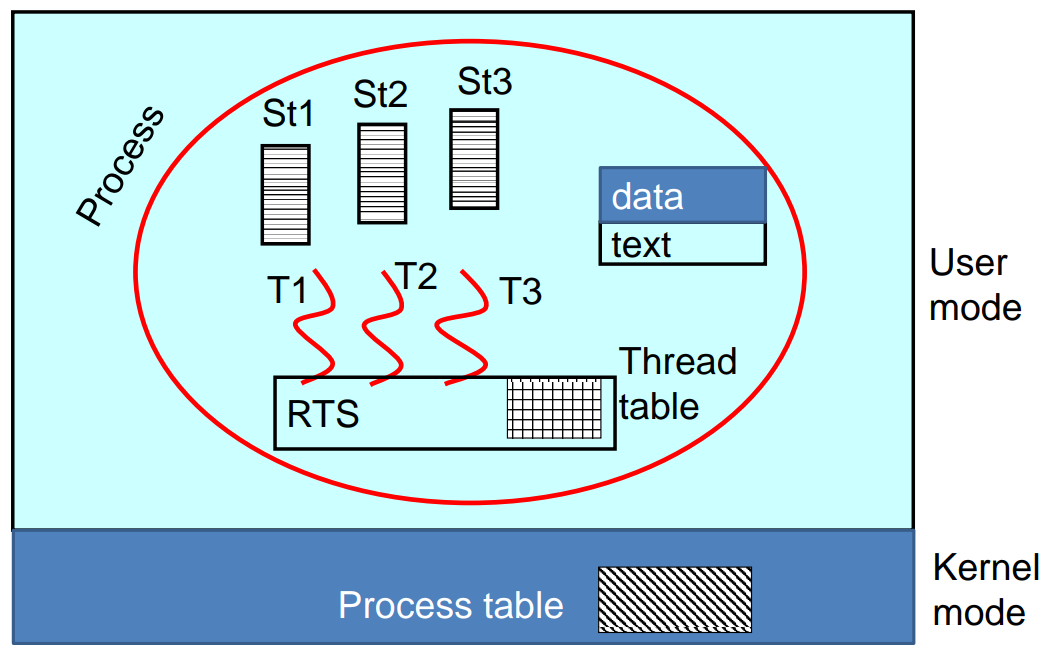
\includegraphics[scale=0.2]{user_level_thread.png}
\end{center}
Per quanto riguarda l'implementazione, l'unica differenza è che la libreria fornisce una istruzione che permette di far partire e fermare il thread, oltre che di fare controlli e pulizia.
\begin{lstlisting}[language=C]
	stub(func, args);
\end{lstlisting}
I principali lati positivi dei user-level thread sono:
\begin{itemize}
	\item Creazione, terminazione e cambio di contesto (cambio di stato) più \textbf{efficienti} in quanto basta una chiamata alla libreria e non al SO
	\item Quando avviene un cambio di contesto l'addressing space rimane lo stesso
	\item Può essere implementato anche in SO che non supportano il multithreading
\end{itemize}

\subsubsection{Kernel-level thread}
In questo caso i thread vengono implementati dal kernel, che conterrà la relativa tabella e gestirà la creazione, terminazione e cambio di contesto. I lati positivi sono che i thread sono effettivamente parallelizzabili e in caso di system call bloccanti si blocca il singolo thread e non l'intero processo.
\begin{center}
	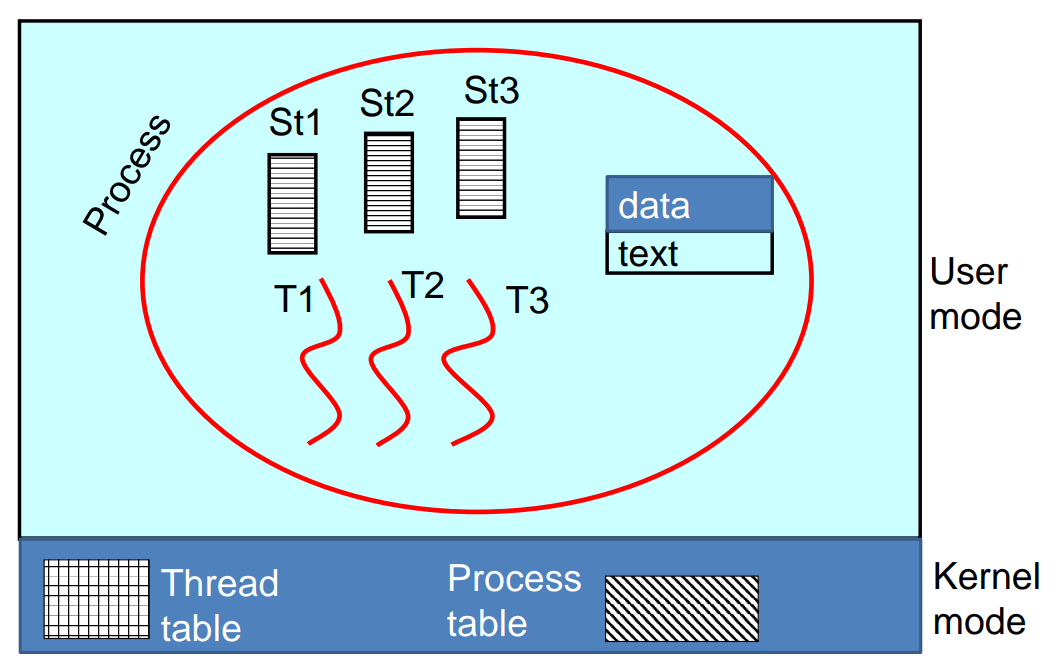
\includegraphics[scale=0.2]{kernel_level_thread.png}
\end{center}
I principali lati negativi sono che ci sarà un costo maggiore per il cambio di contesto dato che sono necessarie delle system call.

\begin{observation}[Asynchronous I/O]
	Un'alternativa ai thread implementati a livello kernel è la gestione di input e output tramite chiamate asincrone.
\end{observation}

\subsubsection{Switch}
Il cambio di contesto di un thread può avvenire per due cause:
\begin{itemize}
	\item \textbf{Volontariamente}:
	\begin{itemize}
		\item \textit{User-level} threads: vengono salvati i registri sul TCB, viene fatto il cambio di stack e  di thread, ripristinati i registri del nuovo thread e \textit{return}
		\item \textit{Kernel-level} threads: identico allo user-level tranne che invece della \textit{return} c'è un'istruzione apposita
	\end{itemize}
	\item A causa di un \textbf{interrupt} o un'\textbf{eccezione} (e.g. timer dello scheduler o interrupt I/O): può essere eseguito in due modi
	\begin{itemize}
		\item \textit{Semplice}: l'interrupt handler salva i registri nello stack, chiama la funzione per eseguire lo switch 
		\item \textit{Veloce}: l'interrupt handler salva i registri sul TCB
	\end{itemize}
\end{itemize}
Il cambio di contesto può generare \textbf{overhead} a causa di:
\begin{itemize}
	\item Salvataggio e ripristino del registri
	\item Gestione dei TCB
	\item Memory cache invalidation
	\item Errori di memoria, quali:
	\begin{itemize}
		\item Address exceptions
		\item Page faults
		\item MMU invalidations
	\end{itemize}
\end{itemize}